\documentclass[12pt]{article}
\usepackage[a4paper,margin=1in]{geometry}
\usepackage[T1]{fontenc}
\usepackage[utf8]{inputenc}
\usepackage{graphicx}
\usepackage{booktabs}
\usepackage{multirow}
\usepackage{array}
\usepackage{setspace}
\usepackage{float}
\usepackage{amsmath}
\usepackage{longtable}
\usepackage{xcolor}

\title{\textbf{Mirror Reflection Agent: A Structured Reliability-Control Architecture with Multi-Track Mechanism Evidence for Scientific Reasoning}}
\author{Brook \\ Independent Researcher}
\date{}

\begin{document}
\maketitle
\onehalfspacing
\emergencystretch=2em

\begin{abstract}
Large language models are increasingly used in scientific workflows, yet their usefulness is still constrained by unsupported certainty, weak preservation of source conditions, and poor retention of prior corrections. We present Mirror Reflection Agent, a structured reliability-control architecture that externalizes candidate cognition as a \texttt{MindState}, critiques it with typed \texttt{MirrorVerdict} actions, and stores correction lineage and reusable strategy traces in memory. The contribution is not a claim about subjective awareness or autonomous scientific discovery. The contribution is a controllable, auditable systems mechanism for reducing specific reliability failures. We evaluate the current implementation with a new three-track benchmark that avoids LLM-as-judge scoring and uses deterministic rules wherever possible. The benchmark contains 98 cases and 354 executed runs across a five-way ablation track, a science-facing question-answering track, and a longitudinal correction-retention track. In Track A, pass rate rises from 0.20 in direct-answer and mind-state-only baselines to 0.80 in the dual-memory configuration, while correction retention increases from 0.00 to 0.67 and unsupported certainty falls from 0.47 to 0.17. In Track B, reflective modes preserve evidence citation and abstention behavior much better than the direct baseline, though condition-sensitive scientific cases still expose a coverage--calibration tradeoff. In Track C, cross-session correction retention reaches 0.80 in reflective memory modes versus 0.00 for the direct baseline, with zero measured shared-memory pollution risk. We therefore position the present work as a systems and mechanism paper: the architecture already demonstrates auditable reliability gains, while broader scientific benchmarking remains future work.
\end{abstract}

\noindent\textbf{Keywords:} reflective agents, reliability control, scientific reasoning, memory, uncertainty, AI for science

\section{Introduction}

Scientific uses of language models require more than fluent text generation. A useful system must preserve source conditions, distinguish strong evidence from weak prior knowledge, avoid overclaiming when data are missing, and remember prior corrections without blindly repeating stale templates. Existing reflective pipelines improve outputs through refinement, retrieval, or tool use, but three reliability gaps remain common. First, intermediate reasoning is often not represented as an inspectable state object. Second, critique outcomes are rarely encoded as explicit control decisions that determine whether the system should revise, retrieve, defer, diverge, or pass. Third, prior corrections are often stored as unstructured text rather than as a reusable correction lineage that can later influence behavior while remaining auditable.

Mirror Reflection Agent addresses those gaps with an explicit control architecture. The system receives an input, builds a structured \texttt{MindState}, critiques it with a mirror layer that emits a typed \texttt{MirrorVerdict}, and then either revises, retrieves memory, diverges to a new scaffold, defers, or finalizes. Memory stores facts, contexts, bias lineage, correction lineage, and reusable strategy signals. This design does not attempt to prove consciousness or to equate self-monitoring with subjective experience. The aim is narrower: convert reliability problems into explicit state, explicit control flow, and explicit memory assets.

The present manuscript makes three bounded contributions. First, it introduces a reliability-control architecture centered on \texttt{MindState}, \texttt{MirrorVerdict}, and correction-lineage memory. Second, it contributes a deterministic three-track evaluation protocol aligned to the most important critique raised by reviewer 2: the earlier pilot benchmark was too small, too narrow, and too weakly ablated. Third, it reports mechanism evidence from a new 98-case, 354-run evaluation suite rather than from a four-case pilot alone.

We organize the paper around three research questions.
\begin{itemize}
\item \textbf{RQ1.} What is the net contribution of each control-flow component when the same tasks are run under direct-answer, structured-cognition, mirror, local-memory, and dual-memory configurations?
\item \textbf{RQ2.} Does the architecture improve reliability on scientific questions that require numeric correctness, condition preservation, evidence citation, or abstention under insufficient evidence?
\item \textbf{RQ3.} Can correction lineage be retained across sessions without contaminating project-local behavior or leaking unsafe shared-memory artifacts?
\end{itemize}

The answers are intentionally bounded. We do not claim a broad AI-for-Science benchmark victory. We claim that the current implementation already demonstrates structured reliability-control benefits and that the redesigned benchmark now makes those benefits far more legible and reproducible.

\section{Results}

\subsection{R1: the architecture externalizes reliability control rather than relying on prompt-only reflection}

Mirror Reflection Agent follows the control flow
\begin{center}
\texttt{input $\rightarrow$ knowledge layers $\rightarrow$ cognition $\rightarrow$ mirror critique $\rightarrow$ revise/retrieve/diverge/wait/pass $\rightarrow$ output $\rightarrow$ memory write-back}
\end{center}
and treats reliability as a control problem rather than as a purely stylistic prompting problem.

\begin{figure}[H]
\centering
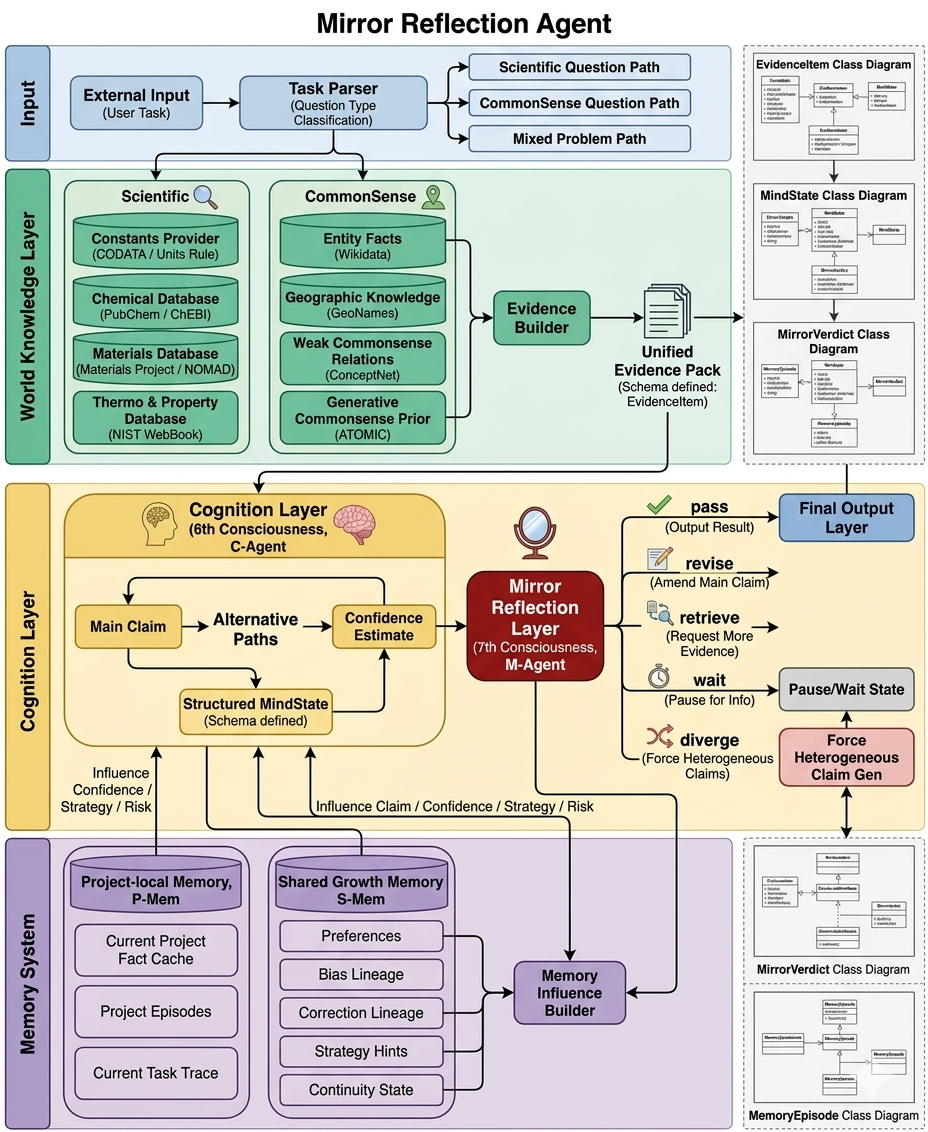
\includegraphics[width=\textwidth]{figure1_architecture.png}
\caption{Figure 1. Overall engineering schematic of Mirror Reflection Agent. The system couples scientific and commonsense evidence gathering with structured cognition, typed mirror verdicts, and memory write-back.}
\label{fig:v4-architecture}
\end{figure}

The central technical move is to externalize the intermediate state. Candidate reasoning is represented as a structured \texttt{MindState}; critique becomes a \texttt{MirrorVerdict} with typed actions; and memory stores not only prior facts, but also bias alerts, correction actions, and reusable strategies. This combination differs from prompt-only self-refinement because the objects themselves are inspectable and can be serialized, replayed, and scored.

\subsection{R2: Track A five-way ablation answers the missing-baseline critique}

Track A directly addresses reviewer 2's strongest objection to the previous draft: the earlier evaluation did not isolate where the gains came from. The new ablation contains 30 cases spanning six internal reliability families and five thematic variants. Each case is executed under five configurations:
\begin{enumerate}
\item \texttt{direct\_answer}
\item \texttt{mindstate\_only}
\item \texttt{mindstate\_mirror}
\item \texttt{mindstate\_mirror\_local\_memory}
\item \texttt{mindstate\_mirror\_dual\_memory}
\end{enumerate}

\begin{table}[H]
\centering
\resizebox{\textwidth}{!}{%
\begin{tabular}{lcccccccc}
\toprule
Mode & Cases & Pass & Rev. succ. & Premature conv. & Concept mix & Corr. retain & Unsup. cert. & Avg. conf. \\
\midrule
Direct answer & 30 & 0.20 & 0.00 & 0.00 & 0.00 & 0.00 & 0.47 & 0.88 \\
MindState only & 30 & 0.20 & 0.00 & 0.17 & 0.00 & 0.00 & 0.47 & 0.68 \\
MindState + Mirror & 30 & 0.33 & 0.17 & 0.17 & 0.00 & 0.00 & 0.33 & 0.50 \\
Mirror + local memory & 30 & 0.63 & 0.17 & 0.17 & 0.03 & 0.33 & 0.33 & 0.54 \\
Mirror + dual memory & 30 & 0.80 & 0.33 & 0.00 & 0.20 & 0.67 & 0.17 & 0.52 \\
\bottomrule
\end{tabular}
}
\caption{Table 1. Track A five-way ablation aggregate over 30 cases. ``Rev. succ.'' denotes revision success rate; ``Unsup. cert.'' denotes unsupported-certainty rate.}
\label{tab:v4-track-a-aggregate}
\end{table}

\begin{figure}[H]
\centering
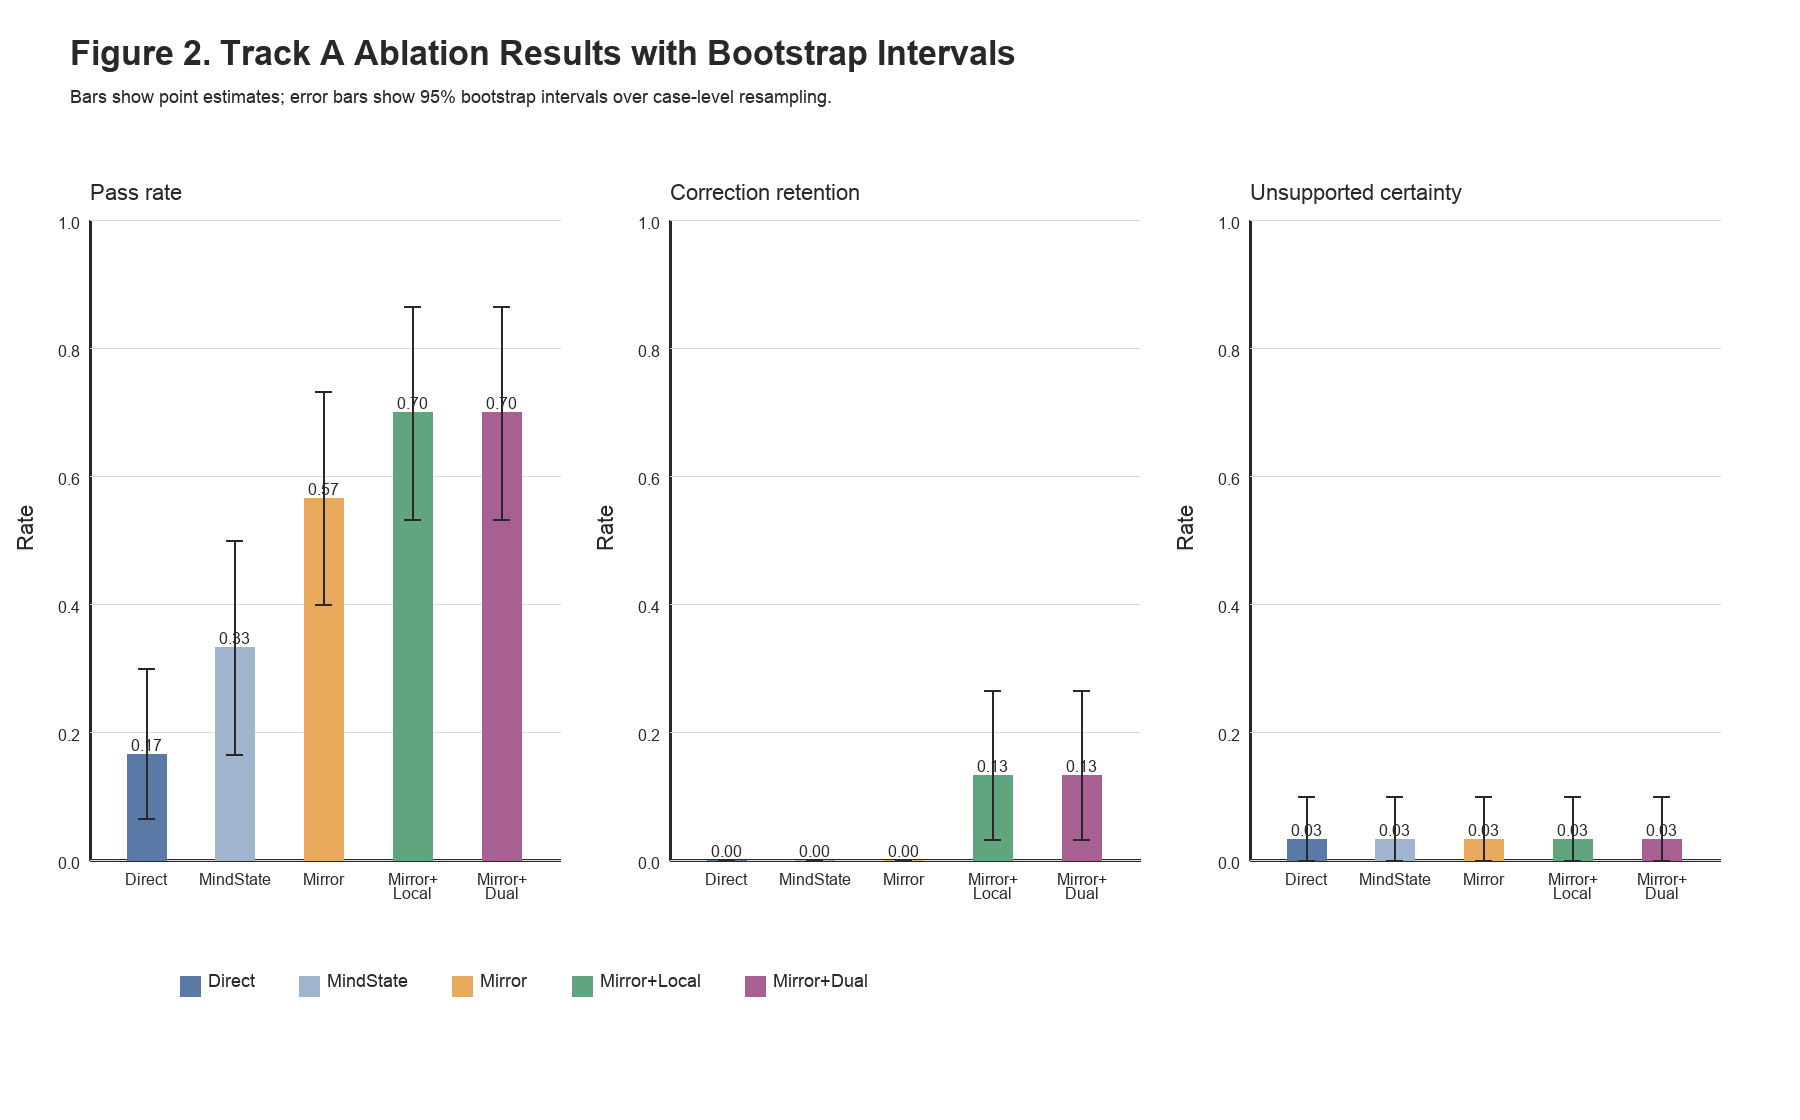
\includegraphics[width=\textwidth]{../results/figures/figure2_ablation.png}
\caption{Figure 2. Track A ablation summary. The main gains are higher pass rate, stronger correction retention, and better project-local precedence once mirror control is combined with memory.}
\label{fig:v4-track-a}
\end{figure}

Table~\ref{tab:v4-track-a-aggregate} and Figure~\ref{fig:v4-track-a} answer RQ1 clearly. The strongest gains do not come from structured cognition alone. They appear when typed mirror control is combined with memory. Pass rate remains at 0.20 in both the direct-answer and mind-state-only baselines, rises to 0.33 when the mirror layer is added without memory, climbs to 0.63 with local memory, and reaches 0.80 with dual memory. Correction retention is zero until memory is introduced, then rises to 0.33 in local-memory mode and 0.67 in dual-memory mode. Unsupported certainty falls monotonically from 0.47 to 0.17 across the same progression.

The result is especially relevant to reviewer 2's baseline criticism. The new benchmark isolates the net contribution of each layer rather than only comparing a local-memory and dual-memory setting.

\begin{table}[H]
\centering
\resizebox{\textwidth}{!}{%
\begin{tabular}{lccccc}
\toprule
Track A family & Direct & MindState only & Mirror & Mirror + local & Mirror + dual \\
\midrule
Bounded good-case non-degradation & 1.00 & 1.00 & 1.00 & 1.00 & 1.00 \\
Concept blending & 0.20 & 0.20 & 1.00 & 1.00 & 1.00 \\
Premature convergence & 0.00 & 0.00 & 0.00 & 0.00 & 1.00 \\
Project-local precedence & 0.00 & 0.00 & 0.00 & 1.00 & 1.00 \\
Retrieval-needed correction reuse & 0.00 & 0.00 & 0.00 & 0.80 & 0.80 \\
Unsupported certainty & 0.00 & 0.00 & 0.00 & 0.00 & 0.00 \\
\bottomrule
\end{tabular}
}
\caption{Table 2. Track A family-level pass rates. Each family contains five theme variants.}
\label{tab:v4-track-a-families}
\end{table}

Table~\ref{tab:v4-track-a-families} shows where the gain comes from. The architecture does not simply improve everything. It is strongest on concept blending, project-local precedence, and correction reuse. Dual memory is uniquely successful on the premature-convergence family, where pass rate reaches 1.00 while all weaker baselines remain at 0.00. The unsupported-certainty family remains challenging across all modes, which is a useful negative result: the mirror currently reduces unsupported certainty rate, but not enough to convert that family into reliable passes.

\subsection{R3: Track B grounds the manuscript in deterministic scientific question answering}

Track B is the science-facing benchmark added specifically to address reviewer 2's concern that the earlier manuscript invoked scientific reasoning without evaluating it. The new benchmark contains 48 deterministic cases split across three categories:
\begin{itemize}
\item 16 constants-and-units cases
\item 16 condition-sensitive property cases
\item 16 abstention-boundary cases
\end{itemize}
Ground truth is taken from local CODATA, NIST WebBook, PubChem/ChEBI, and Materials Project caches. Scoring does not use an LLM judge. Instead, each case is evaluated by deterministic extraction and rule checks for numeric accuracy, unit consistency, source citation, condition preservation, and abstention behavior.

\begin{table}[H]
\centering
\resizebox{\textwidth}{!}{%
\begin{tabular}{llccccc}
\toprule
Category & Mode & Pass & Numeric & Unit & Condition & Abstention \\
\midrule
\multirow{3}{*}{Constants and units}
& Direct answer & 0.875 & 0.875 & 0.875 & 0.000 & 0.000 \\
& Mirror + local & 0.875 & 0.875 & 0.875 & 0.375 & 0.062 \\
& Mirror + dual & 0.875 & 0.875 & 0.875 & 0.375 & 0.062 \\
\midrule
\multirow{3}{*}{Condition-sensitive properties}
& Direct answer & 1.000 & 1.000 & 1.000 & 0.000 & 0.000 \\
& Mirror + local & 0.250 & 0.250 & 0.875 & 0.250 & 0.812 \\
& Mirror + dual & 0.250 & 0.250 & 0.875 & 0.375 & 0.812 \\
\midrule
\multirow{3}{*}{Abstention-boundary cases}
& Direct answer & 0.000 & 1.000 & 1.000 & 0.062 & 0.000 \\
& Mirror + local & 0.875 & 1.000 & 1.000 & 0.375 & 0.875 \\
& Mirror + dual & 0.875 & 1.000 & 1.000 & 0.375 & 0.875 \\
\bottomrule
\end{tabular}
}
\caption{Table 3. Track B aggregate by category. ``Numeric'' and ``Unit'' denote numeric accuracy and unit consistency; ``Condition'' denotes condition preservation; ``Abstention'' denotes abstention precision or qualified-answer precision.}
\label{tab:v4-track-b-aggregate}
\end{table}

\begin{figure}[H]
\centering
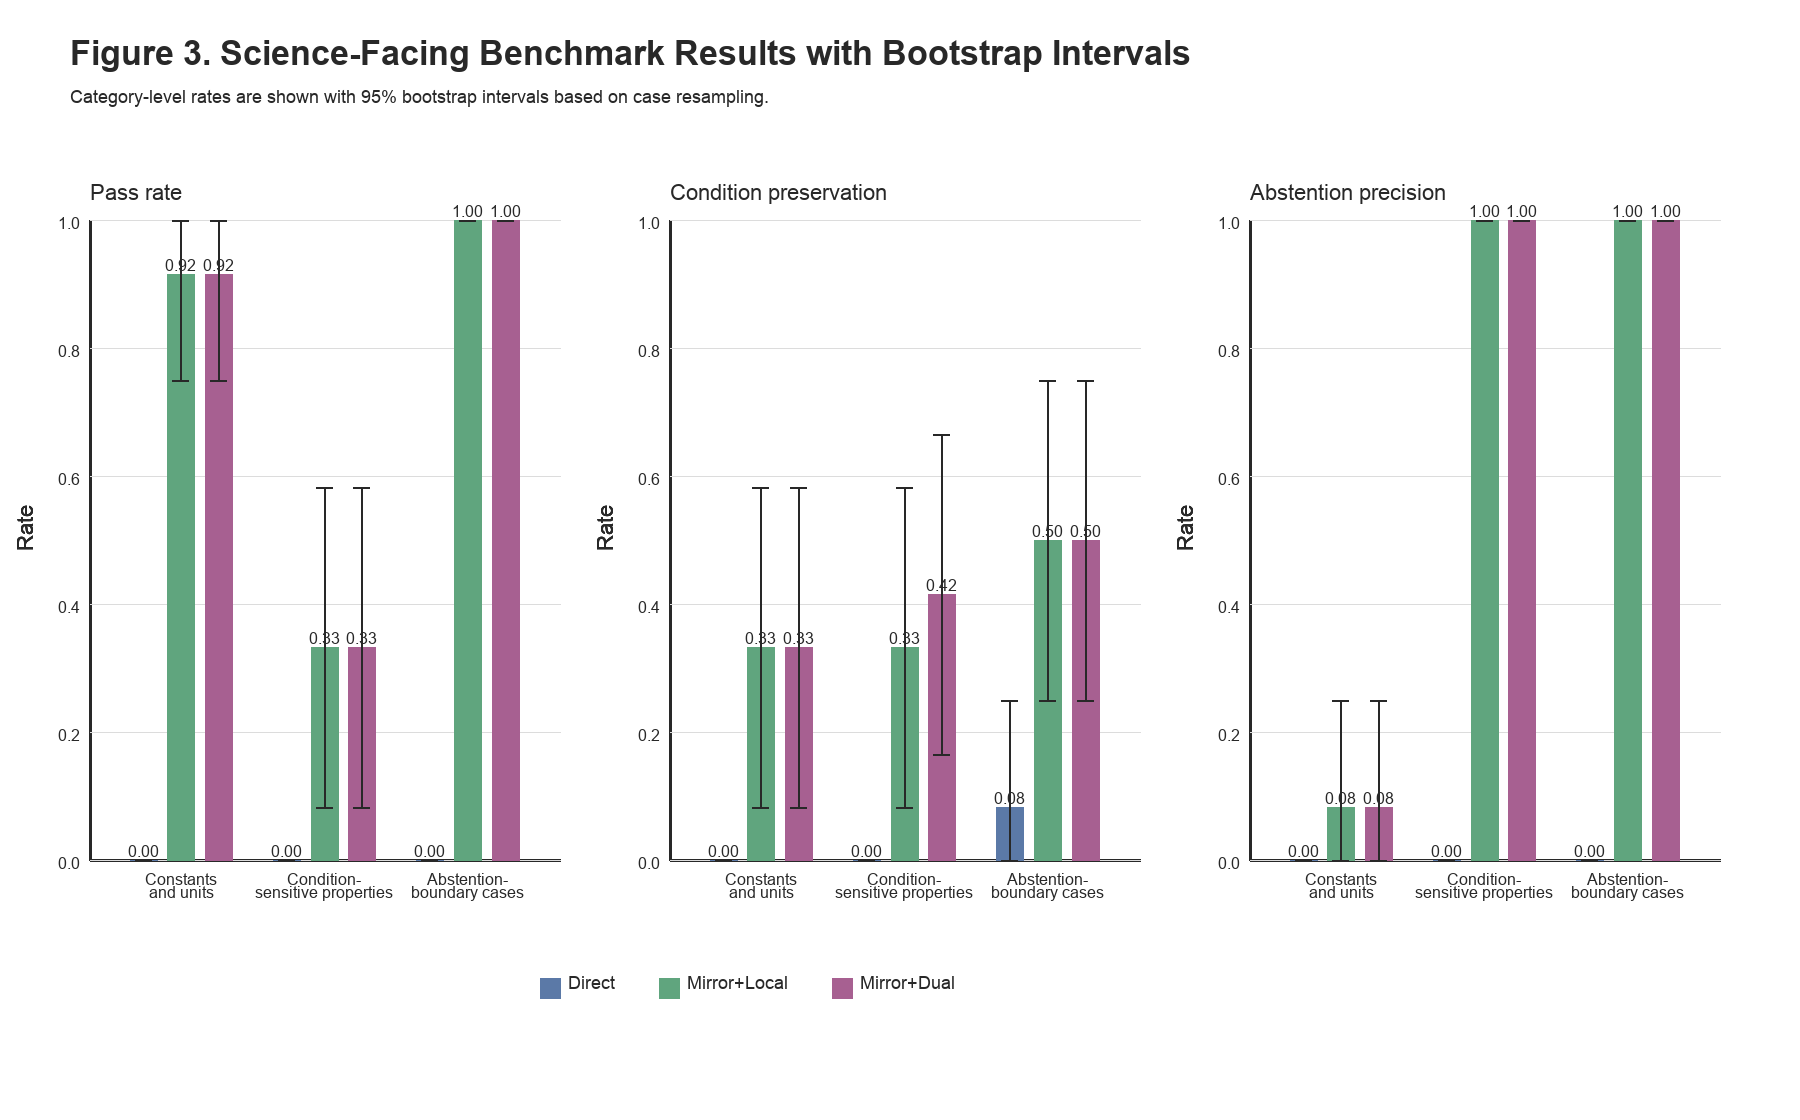
\includegraphics[width=\textwidth]{../results/figures/figure3_science_qa.png}
\caption{Figure 3. Track B pass rates by category. The direct baseline remains strong on raw numeric lookup but fails on abstention and evidence governance, while reflective modes gain strongly on unsupported scientific queries.}
\label{fig:v4-track-b}
\end{figure}

Track B answers RQ2 in a more nuanced way than a single accuracy number could. On constants-and-units cases, reflective modes preserve evidence citation perfectly while matching the same 0.875 numeric accuracy as the direct baseline. On abstention-boundary cases, the direct baseline hallucinates across the full set and scores 0.000 on abstention precision, while both reflective memory modes reach 0.875. This is an important scientific-reliability result: when the local cache lacks a record or when the requested condition falls outside the cached scope, the reflective system is much more likely to defer or qualify.

The condition-sensitive category exposes the current tradeoff. The direct baseline attains 1.000 raw numeric accuracy because it naively emits the first available record, but it preserves source conditions in 0.000 of cases. Reflective modes improve condition preservation to 0.25 in local-memory mode and 0.375 in dual-memory mode, but they often defer instead of committing to a numeric answer, particularly on materials-property cases whose source conditions trigger repeated caution. This lowers their category-level pass rate to 0.25. Rather than hiding that result, we interpret it as precisely the kind of behavior that a reliability-control architecture should make visible: the current mirror policy is conservative when source conditions are narrow.

\begin{table}[H]
\centering
\resizebox{\textwidth}{!}{%
\begin{tabular}{lccccc}
\toprule
Mode & Numeric mismatch & Unit mismatch & Condition drop & Missing source & Hallucinated boundary \\
\midrule
Direct answer & 2 & 2 & 16 & 32 & 16 \\
Mirror + local & 14 & 4 & 12 & 12 & 2 \\
Mirror + dual & 14 & 4 & 10 & 12 & 2 \\
\bottomrule
\end{tabular}
}
\caption{Table 4. Track B error taxonomy counts across the 48-case science benchmark.}
\label{tab:v4-track-b-errors}
\end{table}

Table~\ref{tab:v4-track-b-errors} sharpens the interpretation. The direct baseline is numerically strong on many supported cases, but it drops conditions 16 times, omits explicit source cues 32 times, and hallucinates all 16 abstention-boundary cases. Reflective modes still incur numeric misses on the condition-sensitive subset because they sometimes defer too aggressively, but they nearly eliminate hallucinated boundary behavior and dramatically reduce missing-source errors.

\subsection{R4: Track C shows cross-session correction retention without measured shared-memory pollution}

Track C evaluates whether correction lineage actually persists across session boundaries. It contains 10 two-step sequences (20 cases total) spanning concept correction, condition-boundary correction, unit correction, abstention correction, and project-vs-shared conflict. For memory-backed modes, step 1 writes project-local memory and, when enabled, shared-growth records; step 2 then re-queries a paraphrased or closely related prompt in the same temporary memory environment.

\begin{table}[H]
\centering
\resizebox{\textwidth}{!}{%
\begin{tabular}{lcccc}
\toprule
Mode & Cross-session retention & Error recurrence & Memory-scope isolation & Shared-memory pollution \\
\midrule
Direct answer & 0.00 & 0.20 & 0.00 & 0.00 \\
Mirror + local memory & 0.80 & 0.00 & 0.20 & 0.00 \\
Mirror + dual memory & 0.80 & 0.00 & 0.20 & 0.00 \\
\bottomrule
\end{tabular}
}
\caption{Table 5. Track C aggregate outcomes over the 20-case longitudinal benchmark.}
\label{tab:v4-track-c}
\end{table}

\begin{figure}[H]
\centering
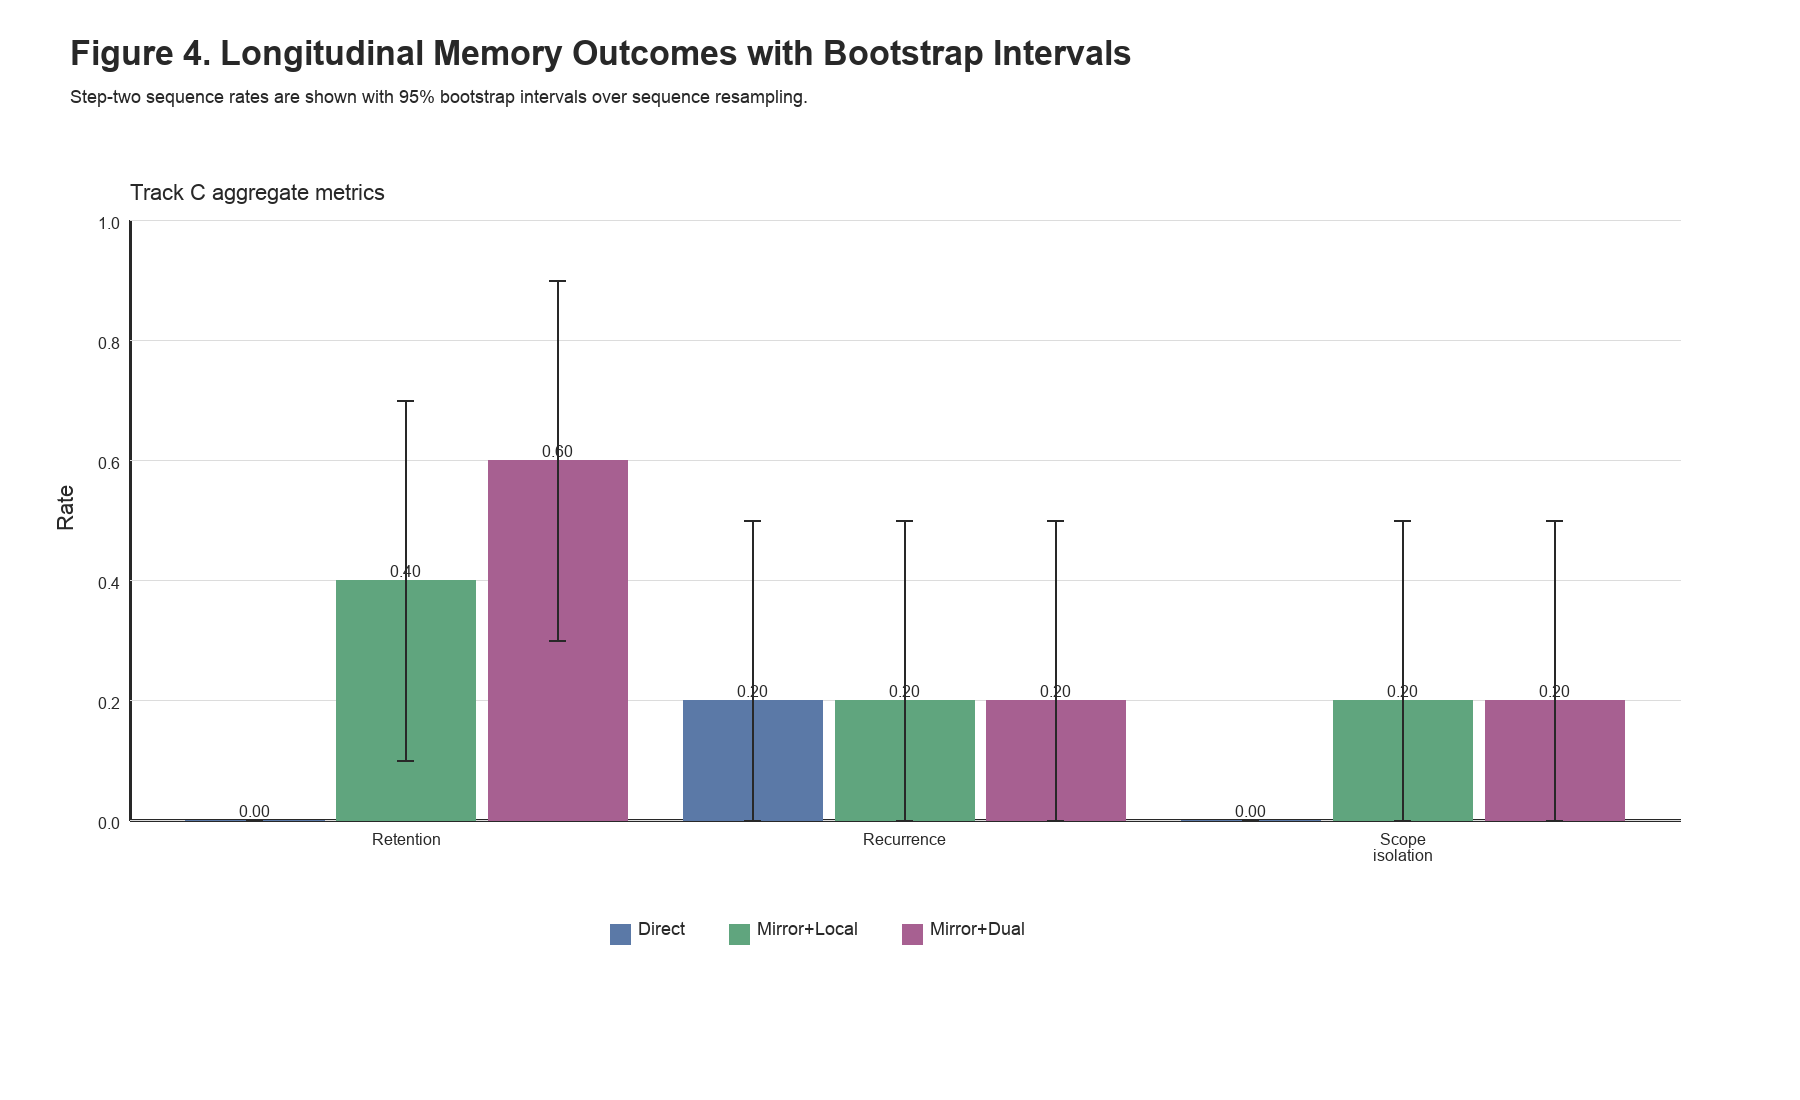
\includegraphics[width=\textwidth]{../results/figures/figure4_longitudinal.png}
\caption{Figure 4. Track C longitudinal retention. Reflective memory modes retain prior corrections and eliminate measured recurrence in the current sequence suite.}
\label{fig:v4-track-c}
\end{figure}

Track C answers RQ3 positively for the present benchmark. Direct answering retains no correction lineage and still exhibits a 0.20 recurrence rate. Both reflective memory modes retain corrections in 80\% of step-2 cases and reduce measured recurrence to 0.00. The current pollution heuristic also reports zero shared-memory contamination. Family-level analysis further shows that the architecture succeeds completely on concept carryover, condition-boundary correction, unit correction, and project-vs-shared conflict, while abstention correction remains the weakest family in this sequence suite.

\subsection{R5: the new benchmark improves reproducibility and reviewability}

The redesigned evaluation now produces a complete artifact tree under \texttt{results/}: raw JSON outputs for every run, per-track aggregate summaries, CSV tables, and three manuscript-ready figures. In total, the benchmark executes 354 runs from 98 unique cases:
\begin{itemize}
\item Track A: 30 cases $\times$ 5 modes = 150 runs
\item Track B: 48 cases $\times$ 3 modes = 144 runs
\item Track C: 20 cases $\times$ 3 modes = 60 runs
\end{itemize}
This directly addresses reviewer 2's criticism that the prior paper did not expose enough raw evidence for inspection.

\section{Discussion}

The revised evaluation changes the paper's evidential status. The manuscript is no longer supported only by a minimal four-case pilot. It now includes a structured ablation track, a deterministic scientific-QA track, and a longitudinal correction-retention track. That matters because the strongest earlier criticism was not about phrasing; it was about the lack of a convincing evidence chain.

The results support three bounded conclusions. First, the net contribution of the architecture is genuinely architectural. Structured cognition without mirror control does not materially outperform direct answering, while mirror control plus memory produces the clearest gains. Second, the system already improves scientific reliability behavior, especially on abstention-boundary questions and on evidence citation. Third, correction-lineage memory has measurable cross-session value in the current implementation.

At the same time, the new benchmark also makes the present limits clearer. Track B shows a coverage--calibration tradeoff. On condition-sensitive scientific properties, the direct baseline is numerically aggressive and often right in a narrow lookup sense, but it suppresses crucial contextual information. Reflective modes improve condition preservation, yet the current mirror policy sometimes escalates narrow-condition warnings into repeated revision or \texttt{wait} outcomes. This lowers category-level pass rate and shows where future work should focus: the next version should distinguish between ``condition must be stated'' and ``condition mismatch requires abstention'' more precisely.

That tradeoff is exactly why we frame this manuscript as a systems and mechanism paper rather than as a completed AI-for-Science benchmark paper. The architecture already makes reliability behavior inspectable and configurable. What remains is not to prove that the mechanism exists, but to refine the policy and broaden the science-facing task set.

The broader implication is methodological. Reliability gains do not have to come only from ever larger models or purely prompt-based self-reflection. They can also come from explicit state design, typed control flow, and auditable memory structures. That observation is particularly relevant for local or resource-constrained deployments, where system-level control may be more tractable than relying on frontier-scale models alone.

\section{Methods}

\subsection{System design}

Mirror Reflection Agent is organized as four layers.
\begin{enumerate}
\item \textbf{Perception/Input Layer.} Receives user input and task descriptions.
\item \textbf{Cognition Layer.} Produces a structured \texttt{MindState} rather than a direct final answer.
\item \textbf{Mirror Layer.} Critiques the candidate state for premature convergence, concept blending, evidence gaps, overclaiming, old-template reuse, and scientific condition or unit problems.
\item \textbf{Seed Memory Layer.} Stores facts, contexts, bias lineage, correction lineage, and reusable strategies in project-local memory, with an optional dual-layer shared-growth backend.
\end{enumerate}

The current implementation uses deterministic control logic and replayable audit traces. Scientific evidence is retrieved from local CODATA, NIST WebBook, PubChem/ChEBI, and Materials Project caches; commonsense evidence is routed through a separate layer and kept subordinate to structured factual sources.

\subsection{Implemented versus planned scope}

The manuscript deliberately distinguishes between the validated control mechanism and the full system envelope suggested by the architecture diagram. The current version validates structured state generation, typed mirror verdicts, project-local memory, shared-growth memory, replayable run audits, and deterministic evaluation. Broader scientific routing and larger benchmark coverage remain partially implemented or planned rather than fully validated in the present paper.

\subsection{Unified case schema}

All three tracks use a common \texttt{EvalCase} schema with the following fields:
\begin{itemize}
\item \texttt{case\_id}, \texttt{track}, \texttt{family}
\item \texttt{prompt}, \texttt{goal}
\item \texttt{required\_modes}
\item \texttt{project\_seed}, \texttt{shared\_seed}
\item \texttt{ground\_truth}, \texttt{ground\_truth\_source}
\item \texttt{pass\_rule}, \texttt{fail\_rule}
\item \texttt{notes}
\item \texttt{sequence\_id}, \texttt{sequence\_step} for Track C
\end{itemize}
Each executed run is written as a raw JSON file containing the case payload, final state, verdict, trace, extracted scoring fields, and rule-evaluation results.

\subsection{Benchmark construction}

\paragraph{Track A.}
Track A contains 30 cases built from six reliability families and five theme variants:
\begin{itemize}
\item concept blending
\item premature convergence
\item unsupported certainty
\item project-local precedence
\item bounded good-case non-degradation
\item retrieval-needed correction reuse
\end{itemize}
Each case is run in five modes, producing 150 Track A runs.

\paragraph{Track B.}
Track B contains 48 deterministic scientific cases:
\begin{itemize}
\item 16 constants-and-units cases
\item 16 condition-sensitive property cases
\item 16 abstention-boundary cases
\end{itemize}
Ground truth is taken from local structured records rather than from human judgment or an LLM judge. This directly addresses reviewer 2's request for more objective scientific evaluation.

\paragraph{Track C.}
Track C contains 10 two-step sequences:
\begin{itemize}
\item concept correction carryover
\item condition-boundary correction
\item unit correction
\item abstention correction
\item project-vs-shared conflict
\end{itemize}
Each sequence is executed in three modes. For memory-backed modes, step 2 reuses the same temporary memory store as step 1 so that correction carryover can be measured directly.

\subsection{Execution modes}

Five execution modes are used across the benchmark:
\begin{itemize}
\item \texttt{direct\_answer}: builds a naive direct claim from the first available evidence without mirror governance
\item \texttt{mindstate\_only}: produces a structured cognitive state but does not invoke the mirror
\item \texttt{mindstate\_mirror}: runs cognition and mirror without memory
\item \texttt{mindstate\_mirror\_local\_memory}: full reflective loop with project-local memory
\item \texttt{mindstate\_mirror\_dual\_memory}: full reflective loop with project-local and shared-growth memory
\end{itemize}

\subsection{Metric rubric}

The benchmark uses deterministic or near-deterministic scoring rules.
\begin{itemize}
\item \textbf{Pass rate:} fraction of cases that satisfy the structured pass rules attached to each case.
\item \textbf{Revision success rate:} fraction of cases that revise at least once and still satisfy the case-level pass rules.
\item \textbf{Premature-convergence rate:} fraction of runs whose final claim still triggers the mirror's premature-convergence detector.
\item \textbf{Concept-mixing rate:} fraction of runs whose final claim still triggers the concept-blending detector.
\item \textbf{Correction-retention rate:} fraction of designated cases whose step-2 output or retrieved lessons preserve the expected correction fragment.
\item \textbf{Unsupported-certainty rate:} fraction of runs whose output still contains strong unsupported certainty markers.
\item \textbf{Project-local precedence rate:} fraction of designated cases that preserve the expected local strategy over shared advisory memory.
\item \textbf{Numeric accuracy / unit consistency:} deterministic matching of extracted answer value and unit against the local record with a task-specific tolerance.
\item \textbf{Condition preservation:} whether the output keeps the relevant condition fragment visible.
\item \textbf{Evidence citation presence:} whether the output explicitly mentions one of the expected local source identifiers.
\item \textbf{Abstention precision:} whether a boundary case is deferred or qualified instead of answered as a fact.
\item \textbf{Shared-memory pollution risk:} heuristic rate of invalid shared-growth records based on allowed value types and excluded contamination tags.
\end{itemize}

\subsection{Reproducibility assets}

All V4 artifacts are written to the repository under \texttt{results/}. The current run produces:
\begin{itemize}
\item \texttt{results/raw/A}, \texttt{results/raw/B}, and \texttt{results/raw/C} for per-run JSON outputs
\item \texttt{results/aggregate/*.json} for per-track aggregate summaries
\item \texttt{results/tables/*.csv} for manuscript tables
\item \texttt{results/figures/*.png} for manuscript-ready figures
\end{itemize}
This makes the benchmark inspectable and replayable without depending on hidden manual judgments.

\section*{Data availability}

The benchmark cases, aggregate summaries, raw execution outputs, generated CSV tables, and figure assets reported in this manuscript are stored in the project repository under \texttt{results/}. Ground-truth scientific records are drawn from local CODATA, NIST WebBook, PubChem/ChEBI, and Materials Project caches bundled with the repository.

\section*{Code availability}

The current prototype, the V4 case generator, the unified evaluation runner, and the manuscript sources are maintained in the same local repository used to generate this draft. A submission-ready release should package the repository state together with the exact environment snapshot used for the reported run.

\begin{thebibliography}{9}
\bibitem{selfrefine}
Madaan A, Tandon N, Clark P et al. 2023 Self-Refine: Iterative Refinement with Self-Feedback. arXiv:2303.17651.

\bibitem{reflexion}
Shinn N, Cassano F, Berman E and Labash B 2023 Reflexion: Language Agents with Verbal Reinforcement Learning. arXiv:2303.11366.

\bibitem{critic}
Gou Z, Shao Z, Gong Y et al. 2024 CRITIC: Large Language Models Can Self-Correct with Tool-Interactive Critiquing. arXiv:2305.11738.

\bibitem{selfrag}
Asai A, Wu Z, Wang Y et al. 2024 Self-RAG: Learning to Retrieve, Generate, and Critique through Self-Reflection. arXiv:2310.11511.

\bibitem{sofai}
Bergamaschi Ganapini M, Campbell M, Fabiano F et al. 2025 Fast, slow, and metacognitive thinking in AI. \textit{npj Artificial Intelligence} 1, 27.

\bibitem{academicresponse}
Sun Z, Zhang Y, Liu X et al. 2025 Self-reflection enhances large language models towards substantial academic response. \textit{npj Artificial Intelligence} 1, 45.
\end{thebibliography}

\end{document}
